\documentclass[12pt,a4paper]{article}
\usepackage{ucs}
\usepackage[utf8x]{inputenc}
\usepackage{amsmath}
\usepackage{graphicx}
\usepackage{wrapfig}

\title{Osnove Mehatronike 1. lab}
\newcommand{\brvjezbe}{1}
\newcommand{\ime}{Niko Višnjić}
\newcommand{\jmbag}{0036449299}
\newcommand{\grupa}{unknown}
\newcommand{\predmet}{Osnove mehatronike} 
\newcommand{\fakultet}{Fakultet elektrotehnike i računarstva Zagreb} 
\newcommand{\zavod}{Zavod za elektrostrojarstvo i automatizaciju } 
\newcommand{\imevjezbe}{Vježba \thesection: Integracija programske podrške za rad
u realnom vremenu i rotacijskog elektromehaničkog sustava SRV02}
\usepackage[hmargin={3.5cm,2.5cm},height=25.5cm]{geometry}
\input{"zaglavlje.tex"}
\setcounter{secnumdepth}{4}

\DeclareMathSizes{12}{12}{12}{12}

\begin{document}
\section{Uvod}
U okviru ove vježbe obavljamo osnovnu integraciju mehatroničkog sustava s osobnim računalom. Pomoću komponenata i sučelja proizvedenih od strane tvrtke Quanser možemo integrirati i testirati mogućnosti i limitacije povezivanja elektromehaničkog rotacijskog sustava SRV02 i osobnog računala koristeći MATLAB/Simulink i Real Time Windows Target komponente. Vježba se sastoji od projektiranja jednostavnog test programa u programskom okruženju MATLAB/Simulink za predviđeni elektromehanički sustav. U nastavku dokumentiramo i opisujemo pokuse te bilježimo dobivene rezultate i naša zapažanja iz dobivenih mjerenja.

\newpage

\section{O Sustavu}


\begin{wrapfigure}{L}{0.5\textwidth}
  	\begin{center}
    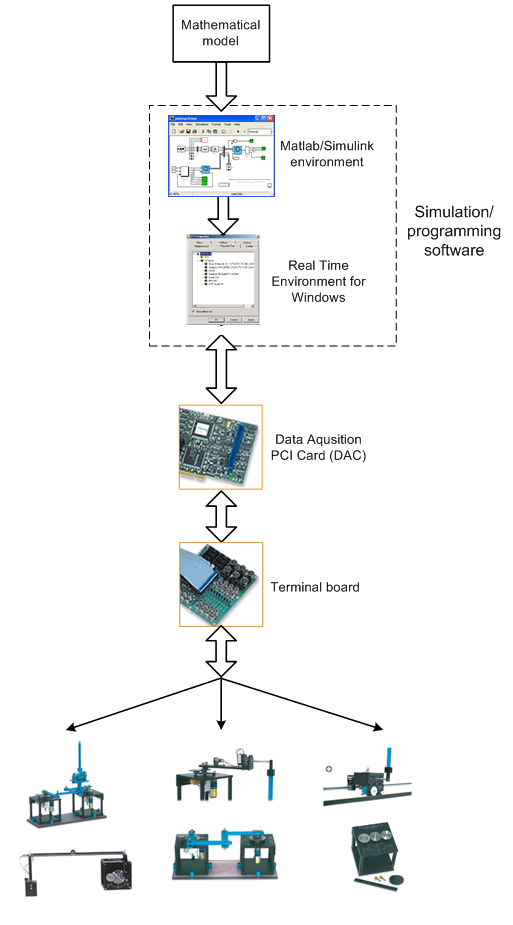
\includegraphics[width=0.35\textwidth]{Lab1_final.png}
  	\caption{Shema povezivanja sustava}
 	\end{center}
    \vspace{-25pt}
\end{wrapfigure}
Prikazano na slici 2.1 imamo generalnu shemu povezivanja zadanog elektromehaničkog sustava sa simulacijskim programima na osobnom računalu. 
Prikazane komponente su sami elektromehanički aktuatori, sučelje između osobnog računala i aktuatora, te programska podrška koju pokrećemo na osobnom računalu. 
Moduli koje koristimo u ovoj vježbi su MultiQ-PCI kartica, koja objedinjuje DAC-ADC pretvarače i sučelje koje koristimo za komunikaciju između PC-a i aktuatora, te sam aktuator u obliku elektromehaničkog rotacijskog sustava SRV02.
Pored navedenih komponenti, potreban nam je izvor napajanja koji će pokretati aktuator, kojeg nalazimo u napajanju UPM 1503. Sve tri korištene komponente su prikazane na slici 2.2.


\begin{verbatim}







\end{verbatim}



\begin{figure}[h]
	\begin{center}
	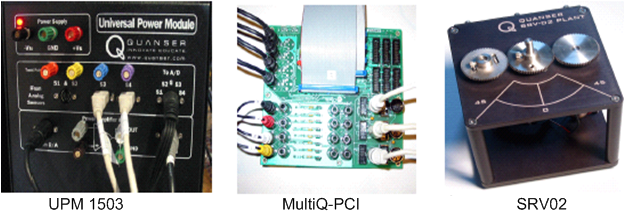
\includegraphics[width=0.8\textwidth] {stuff.png}
    \caption{Komponente korištene u vježbi}
    \end{center}
\end{figure}

\begin{verbatim}






\end{verbatim}


\newpage

\section{Pokusi}
\subsection{Pokus 1: Analogna petlja}
\subsubsection{Opis}
Ovim pokusom provjerava se ispravnost rada analognih ulaza i izlaza te povezanost programskih alata sa sklopovljem sustava. 
\newline
Spajamo MUltiQ-PCI karticu s izvodima kao što je prikazano na slici 3.1.


\begin{figure}[h]
	\begin{center}
	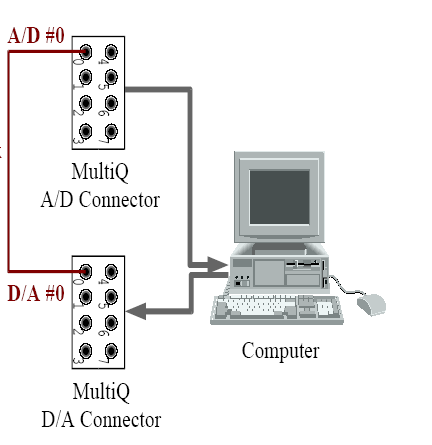
\includegraphics[width=0.3\textwidth] {spoj1.png}
    \caption{Shema spajanja MulitQ-PCI TB}
    \end{center}
\end{figure}

Da bi testirali funkcionalnost MultiQ-PCI sučelja u Simulinku oblikujemo model kao što je prikazano na slici 3.2., te ispravnim postavkama simulacije mjerimo ulazne i izlazne veličine.

\begin{figure}[h]
	\begin{center}
	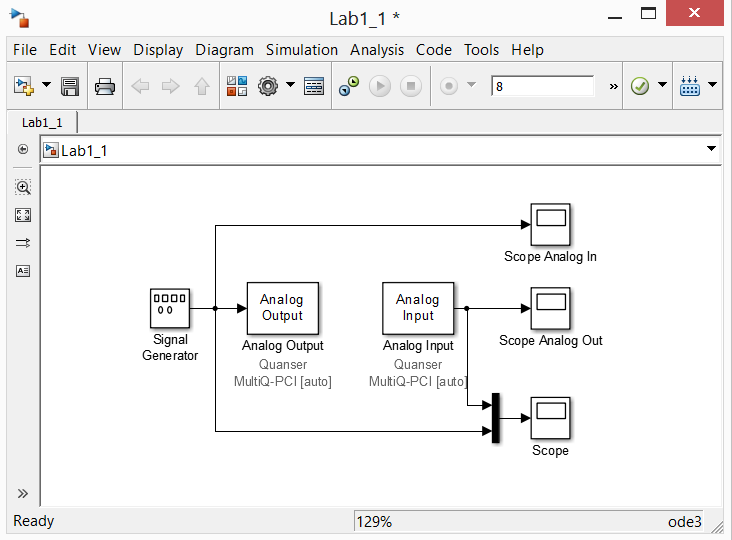
\includegraphics[width=0.8\textwidth] {modelprvi.png}
    \caption{Shema spajanja MulitQ-PCI TB}
    \end{center}
\end{figure}

\newpage
\subsubsection{Rezultati mjerenja}
Snimanjem valnih oblika dobivamo sljedeće grafove.\newline


\begin{figure}[h]
	\begin{center}
	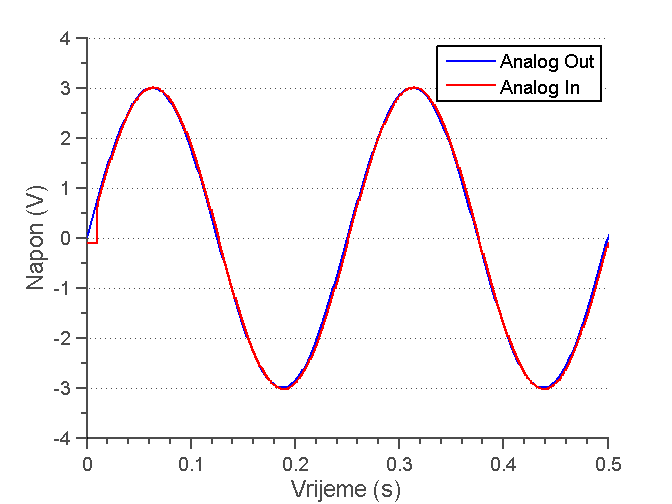
\includegraphics[width=0.8\textwidth] {prvi4.png}
    \caption{Odzivi signala pri $f=4\ Hz$}
    \end{center}
\end{figure}


Pri sinusnom signalu frekvencije $f=4\ Hz$ i ampltude $U=3\ V$ dobivamo vrijednosti izlaznog i ulaznog signala prema slici 3.3. Primjećujemo da ulazni signal relativno vjerno prati izlazni signal koji smo generirali pomoću Matlaba. Naravno, postoji određeno kašnjenje između dvaju signala, što je i za očekivati, jer se generiranje, obrada, pa i sam prijenos signala ne može obaviti trenutačno. Vidimo da je u početnih nekoliko desetina milisekundi snimani ulazni signal jednak nula, što je također posljedica tog kašnjenja. Ukoliko pobliže promotrimo oba signala, što je prikazano na slici 3.4, možemo primijetiti da postoji određeno odstupanje signala.

\begin{figure}[h]
	\begin{center}
	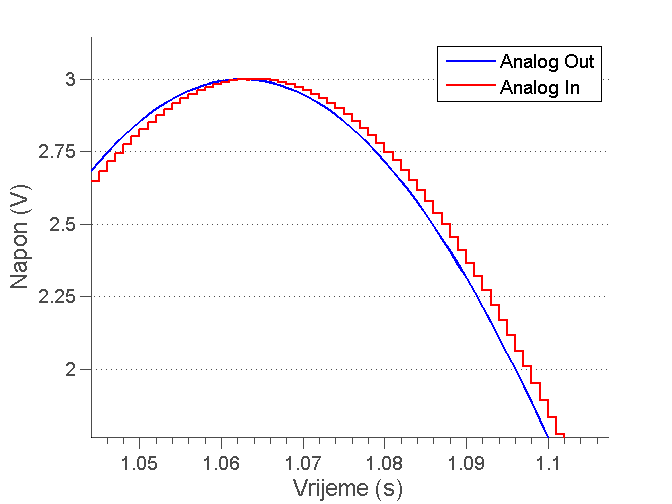
\includegraphics[width=0.8\textwidth] {prvi4closer.png}
    \caption{Odzivi signala pri $f=4\ Hz$, uvećan prikaz}
    \end{center}
\end{figure}

\newpage
To odstupanje je posljedica digitalno-analogne (DAC) i analogno-digitalne (ADC) konverzije unutar MultiQ-PCI kartice prije odašiljanja signala na analogni izlaz, odnosno kod obrada signala s analognog ulaza u format prihvatljiv računalu. Signal Analog In je stepeničast što je posljedica diskretizacije ulaznog analognog signala. Treba primijetiti da signal Analog Out, kojeg snimamo u ovom pokusu, nije signal koji izlazi iz MultiQ-PCI analognog izlaza, već signal kojeg generira funkcija sinusa unutar Matlaba. Sam signal koji izlazi iz analognog izlaza također podliježe konverziji iz digitalnog u analogni oblik, te po svojoj prirodi je diskretan prije konverzije.\newline

Primjećujemo da kod signala frekvencije $f=4\ Hz$ odstupanje uvjetovano diskretizacijom je relativno zanemarivo. Promotrimo li slike 3.5 i 3.6 gdje imamo ulazne signale frekvencije $f_2=16\ Hz$, odnosno $f_3=38\ Hz$, to neće biti slučaj.\newline

Kao što je i za očekivati, vjerodostojnost našeg očitanog signala opada s povećanjem frekvencije promatranog signala. Znamo da je frekvencija očitavanja (eng. sampling time) ADC modula našeg MultiQ-PCI sučelja ostala nepormjenjena, time je preciznost očitanog signala opala kada je signal viših frekvencija. Tako nastalu pogrešku u signalu nazivamo kvantizacijskom pogreškom.\newline

\newpage
\begin{figure}[!ht]
	\begin{center}
	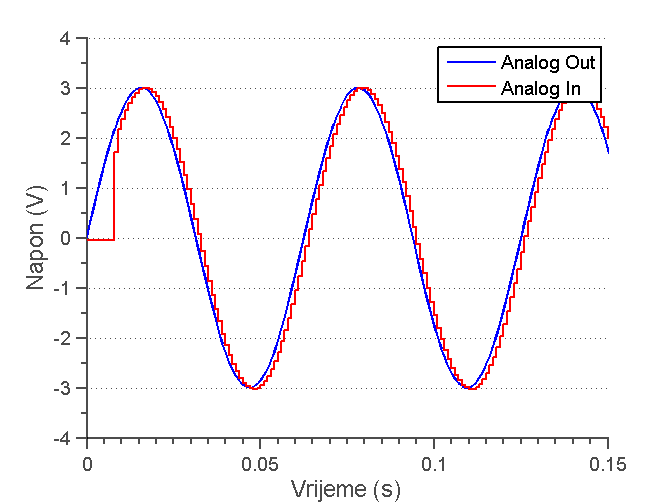
\includegraphics[width=0.8\textwidth] {prvi16.png}
    \caption{Odzivi signala pri $f=16\ Hz$}
    \end{center}
\end{figure}


\begin{figure}[!ht]
	\begin{center}
	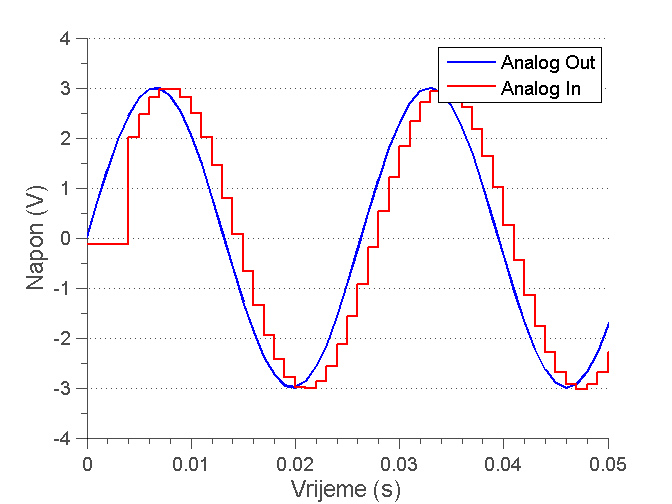
\includegraphics[width=0.8\textwidth] {prvi38.png}
    \caption{Odzivi signala pri $f=38\ Hz$}
    \end{center}
\end{figure}

\newpage
\subsubsection{Opažanja i zaključci}
Proučavanjem navedenih rezultata možemo odgovoriti na nekoliko bitnih pitanja u dosegu ovog pokusa.

Kako senzori, tako motori, pa i ljudi, svi baratamo analognim (realnim) veličinama. Da bi mogli ostvariti bilo kakav oblik komunikacije digitalnog računala i vrijednosti koje su zapisane u digitalnom formatu i okolice, koja barata samo u analognim veličinama, moramo imati način kako pretvoriti digitalne veličine u analogne i obrnuto. 
Tu uviđamo važnost analognih izlaza i analognih ulaza koji su nam primarni način komunikacije s realnim svijetom. Njihovu funkcionalnost ostvarujemo digitalno-analognim (DAC), te analogno-digitalnim (ADC) pretvornicima.

Ovim pokusom uvjerili smo se da su frekvencija promatranog signala i frekvencija očitavanja, kojoj maksimum ovisi samo o našoj opremi, najvažniji parametri pri korištenju analognih ulaza i izlaza. Frekvencija nam određuje koliko dobar rezultat možemo dobiti za određena mjerenja, te time i gdje možemo upotrijebiti naše komponente i da li ih uopće možemo upotrijebiti sa zadovoljavajućim učinkom.
Pored frekvencije, iznosi napona i struja su vrijednosti na koje moramo obratiti pozornost ukoliko ne želimo preopteretiti komponente mehatroničkog lanca.

\newpage

\subsection{Pokus 2: Testiranje mjernih članova SRV02 modula}
\subsubsection{Opis pokusa}

\begin{figure}[!ht]
	\begin{center}
	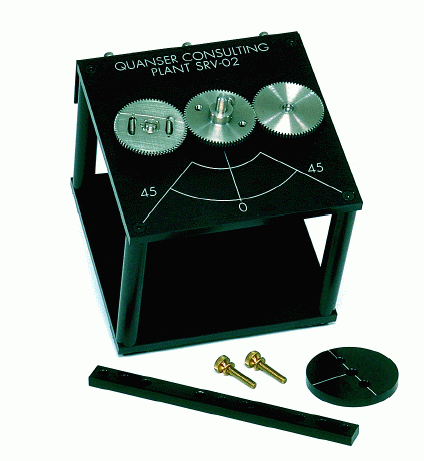
\includegraphics[width=0.7\textwidth] {SRV02.png}
    \caption{SRV02 eletromehanički modul}
    \end{center}
\end{figure}

U ovom pokusu promatramo izlazne signale dva mjerna člana, enkodera i tahogeneratora, pri različitim brzinama vrtnje aktuatora (istosmjernog motora) elektromehaničkog rotacijskog modula SRV02. Oba mjerna člana mjere brzinu vrtnje $n\ [RPM]$

Tahogenerator (MicroMo 2356S006 Motor and Tach Combination) je mali istosmjerni stroj, kojemu je inducirani napon proporcionalan brzini vrtnje. Kako je on direktno spojen na unutarnju osovinu motora, njegovo očitanje daje brzinu vrtnje rotora motora $n_M$.

Enkoder (USDigital Optical Kit Encode) koji koristimo je rotacijski inkrementalni optički enkoder. Na svojem izlazu daje slijed impulsa čiji je broj u jedinici vremena (frekvencija "brojanja") proporcionalan brzini vrtnje. Treba imati na umu da enkoder očitava brzinu vrtnje pogonske osovine $n_L$ (eng. load shaft).\newline

Za ovaj pokus spajamo komponente kao što je prikazano na slici 3.8.
\newpage

\begin{figure}[ht]
	\begin{center}
	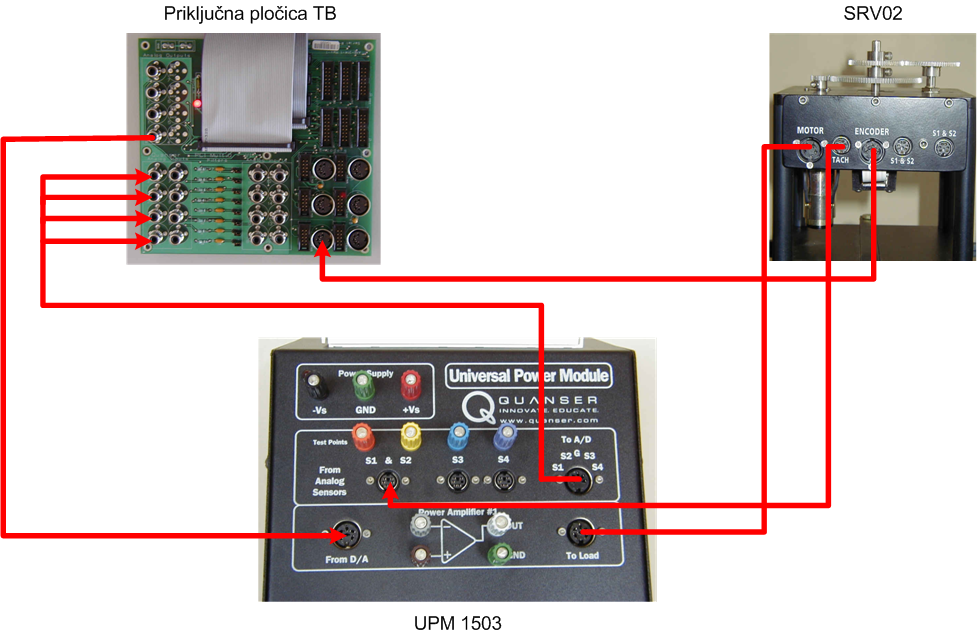
\includegraphics[width=0.8\textwidth] {spoj2.png}
    \caption{Shema spajanja komponenta za pokus 2}
    \end{center}
\end{figure}

Nakon što smo fizički povezali MultiQ-PCI sučelje, napajanje UPM 1503 te elektromehanički modul SRV02, generiramo Simulink model pomoću kojega ćemo upravljati mehatroničkim sustavom i bilježiti njegove ulazne veličine. Simulink model je prikazan na slici 3.9.

\begin{figure}[ht]
	\begin{center}
	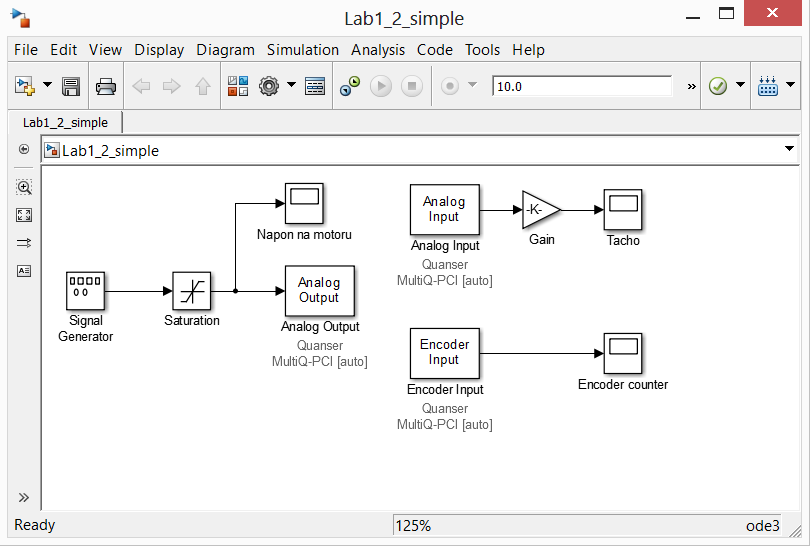
\includegraphics[width=0.8\textwidth] {model2simple.png}
    \caption{Simulink shema za drugi pokus}
    \end{center}
\end{figure}


\subsubsection{Rezultati mjerenja}

Namještanjem napona napajanja, odnosno izlazne analogne veličine, na polovinu iznosa nazivnog napona motora $U_a=3\ V$ te odabirom generiranja pravokutnog signala frekvencije $f=10\ Hz$, dobivamo odzive signala prema sljedećim grafovima.

\begin{figure}[ht]
	\begin{center}
	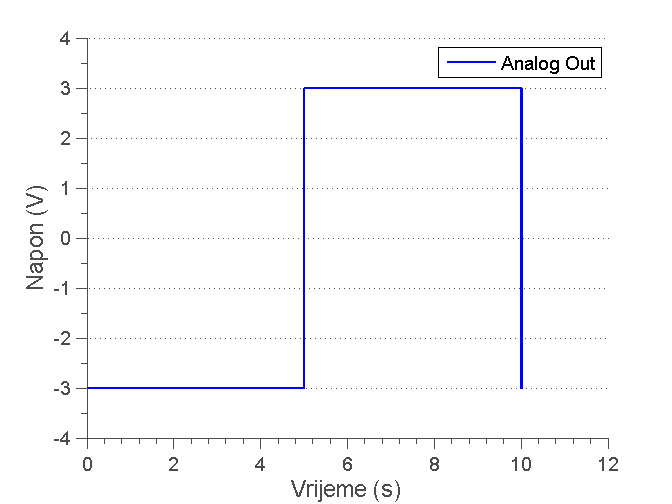
\includegraphics[width=0.8\textwidth] {naponm.png}
    \caption{Napon na motoru $U_a$}
    \end{center}
\end{figure}

Primjećujemo da se prvih pet sekundi motor okreće u obrnutom smjeru rotacije jer mu je narinut negativni napon $U_a$, da bi se nakon pet sekundi promjenio u “pozitivan” smjer rotacije. Nakon deset sekundi simulacije prestaje, te se analogna izlazna veličina postavlja na pretpostavljenu vrijednost 0.

\begin{figure}[!h]
	\begin{center}
	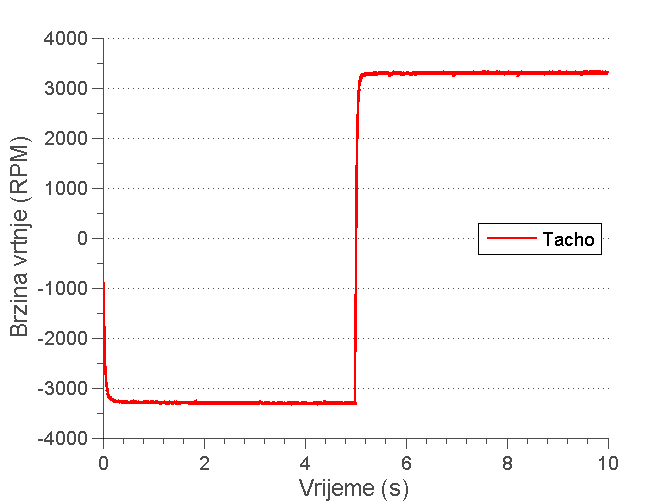
\includegraphics[width=0.8\textwidth] {tachoRPM.png}
    \caption{Signal na izlazu iz tahogeneratora}
    \end{center}
\end{figure} 

\newpage

Na slici 3.11 možemo vidjeti izlaz iz tahogeneratora. Kako bi dobili ovakav signal koji je izražen u okretajima u minuti (eng. rounds per minute, RPM) moramo postaviti Gain funkciju koja je prikazana na Simulink modelu (slika 3.9) na iznos 1000/1.5. Razlog toj preinaci očitanja je što tahogenerator daje na svojem analognom izlazu napon iznosa 1.5 mV po okretaju po minuti, odnosno $U_{tacho}=\frac{1.5\ mV}{1000\ RPM} $. S ovom korekcijom dobivamo stvaran iznos brzine vrtnje motora (osovine rotora) $n_M \approx 3200\ RPM$.\newline

Pogledamo li sada izlaz iz enkodera, koji je prikazan na slici 3.12., primjećujemo da nam on ne prikazuje okretaje u minuti. Što dobivamo pomoću enkoder modula je 24-bitni broj (count), odnosno zbroj reda impulsa generiran u enkoderu, koji se interno sprema na određenu lokaciju na MulitQ-PCI kartici.

Također, valja primijetiti da se Tahogenerator i enkoder rotiraju u suprotnim smjerovima, što je posljedica činjenice da se nalaze na serijski povezanim zupčanicima.

\begin{figure}[!h]
	\begin{center}
	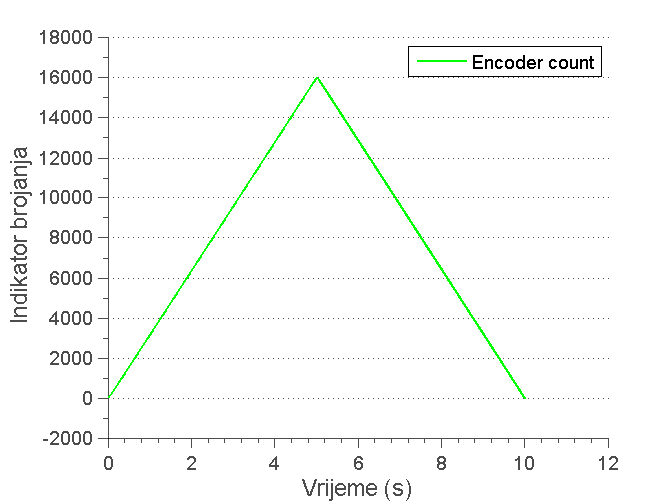
\includegraphics[width=0.8\textwidth] {encoderCnt.png}
    \caption{Signal na izlazu iz enkodera}
    \end{center}
\end{figure}

\subsubsection{Opažanja i zaključci}
Da bi iz ovog broja generiranog pomoću enkodera dobili informaciju o okretajima u minuti, moramo napraviti par preinaka na našem prijašnjem Simulink modelu.\newline

Do rješenja možemo stići na dva načina.
Prvi ukljućuje deriviranje vrijednosti dobivene zbrajanjem po vremenu, gdje nam je iznos po kojemu deriviramo vrlo malen, no ipak različit od nule. 
Drugim načinom dijelimo trenutnu vrijednost zbroja s trenutnim iznosom vremena, gdje moramo postaviti vrijednost vremena na nula nakon što promijenimo smjer okretanja motora, odnosno nakon pet sekundi. Na slici 3.13 možemo vidjeti oba načina dolaženja do željenog oblika izlaza iz enkodera. \newpage

\begin{figure}[!h]
	\begin{center}
	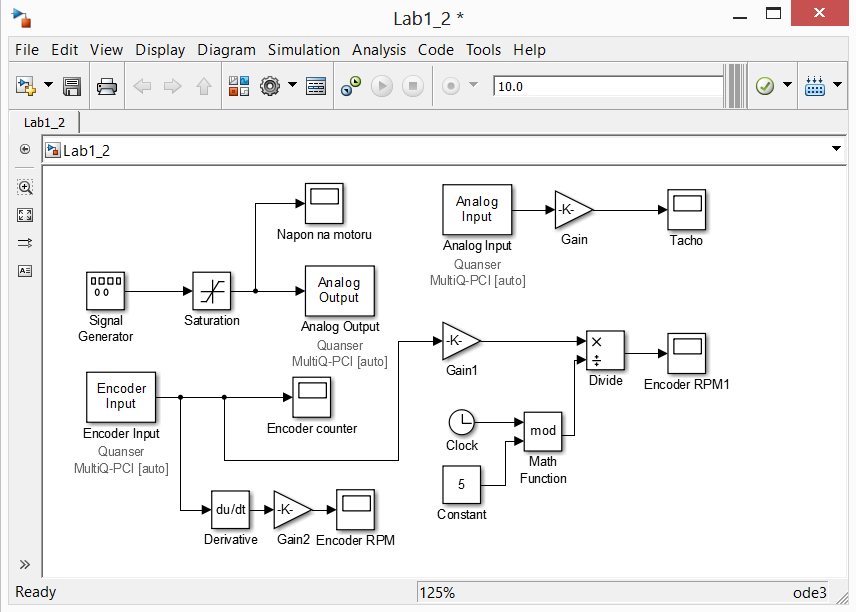
\includegraphics[width=0.8\textwidth] {model2full.png}
    \caption{Proširena Simulink shema za drugi pokus}
    \end{center}
\end{figure}

Primjetimo da u oba rješenja moramo koristiti Gain funkciju s vrijednosti multiplikacije namještenu na 60/4096. Razlog za takvu preinaku je što enkoder u punom okretaju generira točno 4096 impulsa svojem brojaču. S obzirom da već dijelimo, odnosno deriviramo iznos brojača s jedinicom vremena koja je izražena u sekundama, da bi dobili kolika je brzina vrtnje u okretajima u minuti moramo množiti još s 60, odnosno po formuli

\begin{center}
$n_L=\frac{ X_{impulsa} \times 60}{ 4096 \times T_{impulsa}}\ [o/min]$
\end{center}

Kada smo uključili navedene preinake u naš model dobivamo nove odzive signala iz enkodera prema slikama 3.14 i 3.15,  za model s derivatorom, odnosno prema slici 3.16 za rješenje pomoću dijeljenja s proteklim vremenom.
\newpage

\begin{figure}[!h]
	\begin{center}
	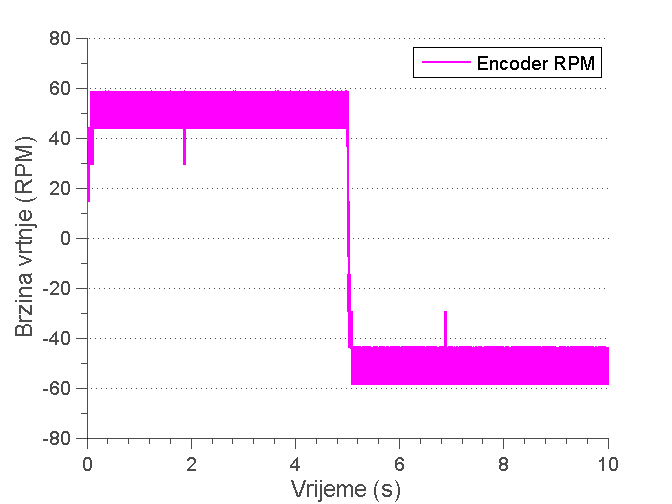
\includegraphics[width=0.8\textwidth] {encoderRPM.png}
    \caption{Signal enkodera u RPM pomoću derivatora}
    \end{center}
\end{figure}

\begin{figure}[!h]
	\begin{center}
	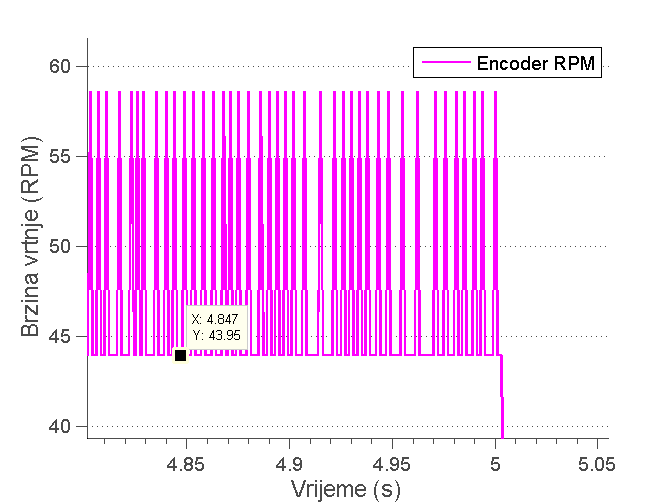
\includegraphics[width=0.8\textwidth] {encoderRPMclose.png}
    \caption{Signal enkodera u RPM pomoću derivatora, uvećan prikaz}
    \end{center}
\end{figure}

\newpage

\begin{figure}[!t]
	\begin{center}
	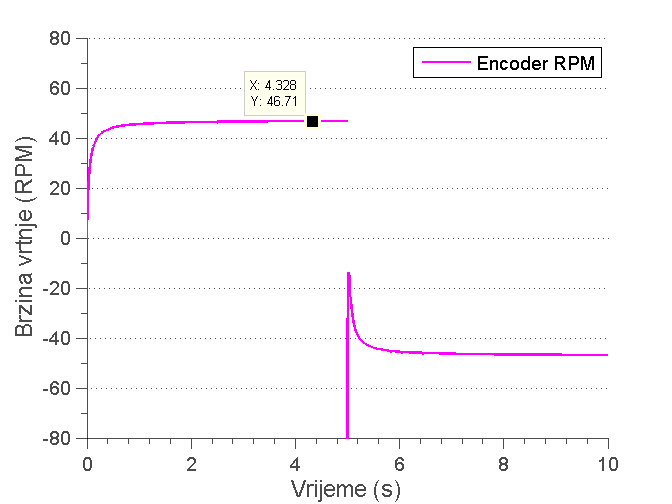
\includegraphics[width=0.8\textwidth] {encoderRPM1.png}
    \caption{Signal enkodera u RPM pomoću dijeljenja}
    \end{center}
\end{figure}


Primjećujemo da imamo neznatno odstupanje kod signala s deriviranjem od vrijednosti očitanih pomoću tahogeneratora.

Pogledamo li na sliku 3.7. možemo vidjeti i vanjsku osovinu motora s zupčanikom. U našem pokusu koristili smo SRV02 modul u konfiguraciji visokog prijenosnog omjera, u kojemu je zupčanik na pogonskoj osovini pet puta veći od vanjskog zupčanika motora. Time dobivamo prijenosni omjer od $5:1$. Nadalje, u unutrašnjoj konstrukciji motora se koristi planetarni prijenosnik koji prenosi okretaje s unutarnje osovine motora na vanjsku. Planetarni prijenosnik u motoru doprinosi s prijenosnim omjerom od $14:1$.

Napominjem još jednom da tahogenerator očitava brzinu vrtnje motora $n_m$, odnosno unutarnje osovine motora.\footnote{Istaknuto iz razloga što su određene osobe izgubile oko sat vremena života tražeći gdje im se brzina vrtnje gubi za aproksimativno 13,47 puta. Do te brojke se došlo računanjem na temelju vizualnih aproksimacija brzine vrtnje pojedinih zupčanika. Bilo bi vrlo uviđajno da se to napomene i u zadacima za izvještaj.}
Stoga, da bi mogli uspoređivati brzinu vrtnje enkodera i brzinu vrtnje tahogeneratora, odnosno odnosno pogonske osovine $n_L$ i motora $n_M$, moramo ih uspoređivati s prijenosnim faktorom $5\times14=70$, odnosno izraženo formulom

\begin{center}
$\tfrac{n_L}{n_M} = \tfrac{1}{70}$
\end{center}

\begin{verbatim}


\end{verbatim}
Zaključujemo da tahogenerator i enkoder zadovoljavajuće dobro određuju brzinu i smjer okretanja motora, odnosno pogonske osovine.


\end{document}

%Na vlastitu odgovornost...
